\section{Piecewise Quadratic Model}

In this section, we will examine the dynamics of a piecewise quadratic model.
Starting with a model with 4 branches and symmetry, like in \Cref{sec:og.full}.
After that, we will reduce the model to just two branches using symmetry.

\subsection{Full Model}

The full model is the map $x \mapsto f(x) \mod 6$.
Where $f$ is given by the following collection of equations.
\begin{align}
    f(x) & = \begin{cases}
        g(x) & \text{if } r(x) < 3 \\
        g(x) + 3 & \text{else}
    \end{cases} \label{equ:quad.full.f} \\
    g(x) & = \begin{cases}
        a_L \cdot s_L(x)^2 + b_L \cdot x + c_L & \text{if } s(x) < \frac{3}{2} \\
        a_R \cdot s_R(x)^2 + b_R \cdot x + c_R & \text{else}
    \end{cases} \label{equ:quad.full.g}
\end{align}

\Cref{equ:quad.full.f} causes the disontinuity in the middle at $x = 3$.
It also makes sure, the symmetry $f(x + 3) \equiv f(x) + 3 \mod 6$ is true.
Each half of the model is then governed by \Cref{equ:quad.full.g}.
Here all the 6 parameters $a_L, a_R, b_L, b_R, c_L,$ and $c_R$ act.

\Crefrange{equ:quad.full.s}{equ:quad.full.sr} provide adjusted values of x for either choosing between branches in both halves or substituting in the quadratic formulas of each branch.
\begin{subequations}
\begin{align}
    s(x) & = x \mod 3 \label{equ:quad.full.s} \\
    s_L(x) & = s(x) - \frac{3}{4} \\
    s_R(x) & = s(x) - \frac{9}{4} \label{equ:quad.full.sr}
\end{align}
\end{subequations}

\subsection{Variation of Single Parameters}

We start by examining the behavior of the quadratic model under variations of single parameters like $a_L, a_R, b_L, b_R, c_L,$ and $c_R$.

\subsubsection{Fixing $a_L = a_R = 1, b_L = b_R = 0$}

\Cref{fig:quadratic.full.2d.full} shows a 2D-scan of the periods of the stable cycles.
The parameters $a_L = a_R = 1$ and $b_L = b_R = 0$ are fixed and the parameters $c_L$ and $c_R$ are varied.
Both are varied within the range $[0, 6]$ because beyond that the diagram just repeats infinitely.
The structure in the middle left is enhanced and depicted in \Cref{fig:quadratic.full.2d.z1}.

\begin{figure}
    \centering
    \begin{subfigure}{0.4\textwidth}
        \centering
        \includegraphics[width=\textwidth]{21_Quadratic_mod6/2D_Period_Full/result.png}
        \caption{Full}
        \label{fig:quadratic.full.2d.full}
    \end{subfigure}
    \begin{subfigure}{0.4\textwidth}
        \centering
        \includegraphics[width=\textwidth]{21_Quadratic_mod6/2D_Period_Zoomed1/result.png}
        \caption{Zoomed}
        \label{fig:quadratic.full.2d.z1}
    \end{subfigure}
    \caption{2D Scan of Full Quadratic Model}
\end{figure}

A phenomenon like in the original model could not be found here.
But something very similar happens on the border of these wings.
\Cref{fig:quad.full.Cobwebs} shows the cobwebs along the line marked in \Cref{fig:quadratic.full.2d.z1}.
Before the border, there is one stable cycle with period 8.
This cycle is depicted in \Cref{fig:quad.full.CobwebA} and its symbolic sequence is $\A^3B\C^3\D$.
At the border, there is an area where two cycles coexist.
You cannot see this in the 2D scans above, since it only ever picks up on one cycle.
\Cref{fig:quad.full.CobwebB} shows the coexisting cycles at this border.
In contrast to the original model, the cycle that existed before in \Cref{fig:quad.full.CobwebA}, still exists alongside the new cycle with period 6.
The symbolic sequence of the new cycle is $\A^2\B\C^2\D$.

This is different from the dynamics in the original model in two ways.
First, the cycles before and after the area of coexistence have different periods.
And second, the cycles existing outside the area of coexistence still exist inside the area of coexistence.
In the original model, the cycles existing outside the area of coexistence would disappear at the border and new cycles would emerge inside this area.

\begin{figure}
    \centering
    \begin{subfigure}{0.3\textwidth}
        \centering
        \includegraphics[width=\textwidth]{21_Quadratic_mod6/Cobweb_A/result.png}
        \caption{Before border}
        \label{fig:quad.full.CobwebA}
    \end{subfigure}
    \begin{subfigure}{0.3\textwidth}
        \centering
        \includegraphics[width=\textwidth]{21_Quadratic_mod6/Cobweb_B/result.png}
        \caption{At border}
        \label{fig:quad.full.CobwebB}
    \end{subfigure}
    \begin{subfigure}{0.3\textwidth}
        \centering
        \includegraphics[width=\textwidth]{21_Quadratic_mod6/Cobweb_C/result.png}
        \caption{After border}
        \label{fig:quad.full.CobwebC}
    \end{subfigure}
    \caption{Cobwebs along marked line}
    \label{fig:quad.full.Cobwebs}
\end{figure}
